\documentclass[tikz,border=5pt]{standalone}
\usepackage{tikz}
\usetikzlibrary{shapes.geometric,arrows.meta,positioning,fit,backgrounds,shadows,decorations.pathreplacing}

\begin{document}
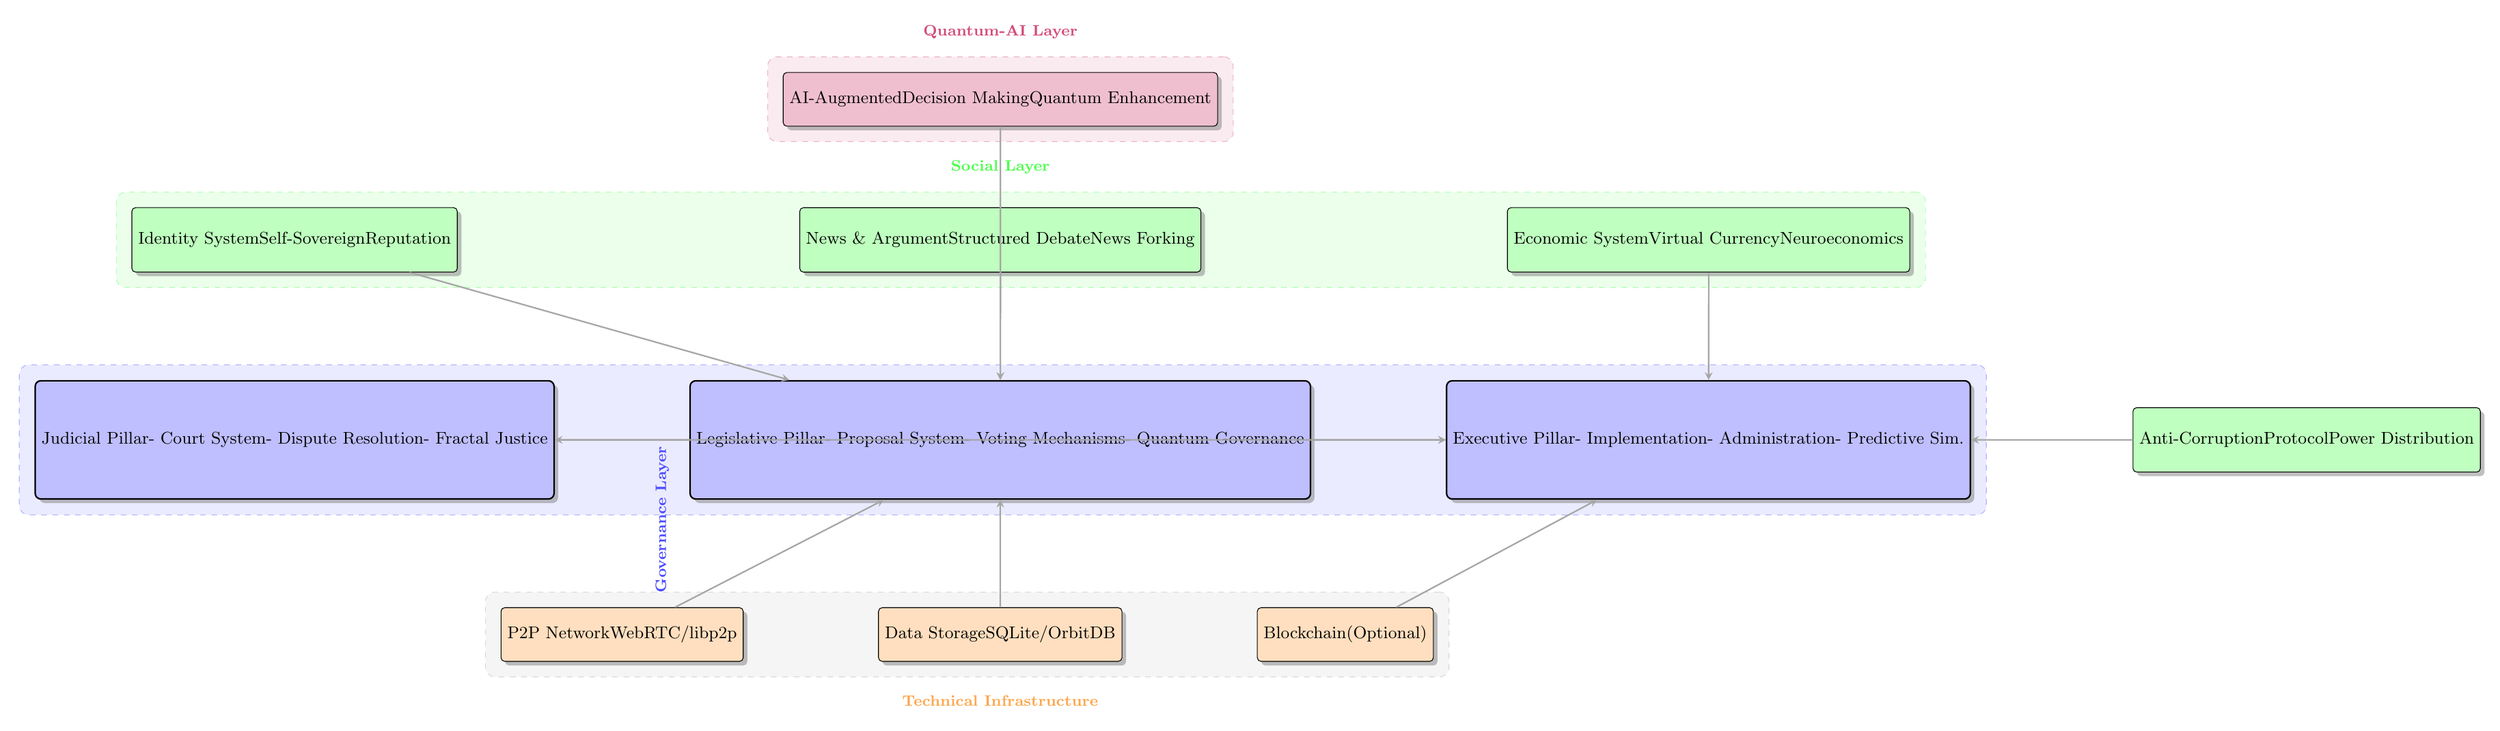
\begin{tikzpicture}[scale=1.5,
    node distance=2.5cm,
    every node/.style={font=\small},
    pillar/.style={rectangle,draw,minimum width=3.2cm,minimum height=2.2cm,fill=blue!25,thick,rounded corners=3pt,drop shadow,text centered},
    system/.style={rectangle,draw,minimum width=2.7cm,minimum height=1.2cm,fill=green!25,rounded corners=2pt,drop shadow,text centered},
    tech/.style={rectangle,draw,minimum width=2.2cm,minimum height=1cm,fill=orange!25,rounded corners=2pt,drop shadow,text centered},
    quantum/.style={rectangle,draw,minimum width=2.5cm,minimum height=1cm,fill=purple!25,rounded corners=2pt,drop shadow,text centered},
    arrow/.style={->,>=stealth,thick,color=gray!70}
]

% Core Infrastructure
\node[tech] (p2p) {P2P Network\\WebRTC/libp2p};
\node[tech,right=of p2p] (storage) {Data Storage\\SQLite/OrbitDB};
\node[tech,right=of storage] (blockchain) {Blockchain\\(Optional)};

% Governance Pillars
\node[pillar,above=2cm of storage] (legislative) {Legislative Pillar\\- Proposal System\\- Voting Mechanisms\\- Quantum Governance};
\node[pillar,left=of legislative] (judicial) {Judicial Pillar\\- Court System\\- Dispute Resolution\\- Fractal Justice};
\node[pillar,right=of legislative] (executive) {Executive Pillar\\- Implementation\\- Administration\\- Predictive Sim.};

% Social Systems
\node[system,above=2cm of judicial] (identity) {Identity System\\Self-Sovereign\\Reputation};
\node[system,above=2cm of legislative] (news) {News \& Argument\\Structured Debate\\News Forking};
\node[system,above=2cm of executive] (economy) {Economic System\\Virtual Currency\\Neuroeconomics};

% AI/Quantum Layer
\node[quantum,above=1.5cm of news] (ai) {AI-Augmented\\Decision Making\\Quantum Enhancement};

% Anti-Corruption
\node[system,right=3cm of executive] (anticorr) {Anti-Corruption\\Protocol\\Power Distribution};

% Background boxes with enhanced styling
\begin{scope}[on background layer]
\node[fill=gray!8,draw=gray!30,dashed,fit=(p2p)(storage)(blockchain),inner sep=8pt,rounded corners=5pt] {};
\node[fill=blue!8,draw=blue!30,dashed,fit=(judicial)(legislative)(executive),inner sep=8pt,rounded corners=5pt] {};
\node[fill=green!8,draw=green!30,dashed,fit=(identity)(news)(economy),inner sep=8pt,rounded corners=5pt] {};
\node[fill=purple!8,draw=purple!30,dashed,fit=(ai),inner sep=8pt,rounded corners=5pt] {};
\end{scope}

% Connections
\draw[arrow] (p2p) -- (legislative);
\draw[arrow] (storage) -- (legislative);
\draw[arrow] (blockchain) -- (executive);
\draw[arrow] (legislative) -- (judicial);
\draw[arrow] (legislative) -- (executive);
\draw[arrow] (judicial) -- (executive);
\draw[arrow] (identity) -- (legislative);
\draw[arrow] (news) -- (legislative);
\draw[arrow] (economy) -- (executive);
\draw[arrow] (ai) -- (legislative);
\draw[arrow] (anticorr) -- (executive);

% Enhanced Labels
\node[below=0.5cm of storage,font=\footnotesize\bfseries,color=orange!70] {Technical Infrastructure};
\node[left=0.5cm of legislative,font=\footnotesize\bfseries,color=blue!70,rotate=90] {Governance Layer};
\node[above=0.5cm of news,font=\footnotesize\bfseries,color=green!70] {Social Layer};
\node[above=0.5cm of ai,font=\footnotesize\bfseries,color=purple!70] {Quantum-AI Layer};

\end{tikzpicture}
\end{document}
